
\chapter{Evaluación y Resultados}

\label{chap6:evaluacion}

\section{Introducción}

En el ámbito de investigación y desarrollo de sistemas \abbr{HAR}
existen dos elementos vitales: la recolección de datos experimentales
y generación del conjunto de entrenamiento. En este capítulo, describimos
de manera general estos elementos en las primeras dos secciones. La
sección \ref{sec6:recoleccion} describe los aspectos relacionados
a la captura de datos, determinando los requisitos mínimos de los
teléfonos móviles utilizados y describiendo el procedimiento guía
para experimentación. Posteriormente, la sección \ref{sec6:clasificacion}
describe los resultados obtenidos al aplicar las técnicas descritas
en la sección \ref{sec44:proceso-se=0000F1ales} para transformar
datos sensoriales a un conjunto de entrenamiento para la clasificación
de actividades humanas. Finalmente, en la sección \ref{sec6:resultados}
los resultados producidos al utilizar el conjunto entrenamiento disponible
son presentados. Esto incluye la validación del modelo construido
con el algoritmo de \emph{Machine Learning} (\abbr{ML}) escogido
que confirma su usabilidad en ambientes productivos. También se expone
la evaluación de los resultados producidos por \emph{\abbr{HARDroid}
}con la aplicación \emph{ActivitySurvey} desarrollada para esta tarea.

\section{Datos Experimentales}

\label{sec6:recoleccion}En base a trabajos precedentes en sistemas
\abbr{HAR}, se han dispuesto datos experimentales para entrenar clasificadores
de actividades humanas tales como en \cite{ReyesOrtiz2013}. Estos
datos están disponibles como fuente para diversos estudios de investigaciones
en este ámbito. 

Sin embargo, los datos de sensores capturados con teléfonos móviles
son escasos. Es por esta razón que este trabajo requirió realizar
una colecta acorde a los objetivos de estudio del mismo. El procedimiento
y los datos recolectados por medio de experimentación se describen
a continuación.

\subsection{Instrumentación}

Como es sabido el desarrollo de \emph{\abbr{HARDroid} }se concreto
completamente para la plataforma \emph{\abbr{Android} }y a continuación
se detallan los rasgos técnicos de las herramientas utilizadas para
su concepción y evaluación.

\subsubsection{Teléfonos inteligentes}

Escoger las herramientas apropiadas para desarrollar un sistema \abbr{HAR}
requiere de la evaluación de dispositivos móviles disponibles en el
mercado teniendo en cuenta los criterios citados en la \secref{sec24:dispositivos-moviles}:
\emph{hardware}, sensores y software de plataforma. En el periodo
de evaluación de este trabajo (2016), la cantidad de teléfonos inteligentes
con sensores de aceleración fue vasta, algunos de los cuales se listan
en la \tabref{tab6:dispositivos} con sus características relevantes.

\begin{table}[h]
\begin{centering}
\begin{tabular}{|l|>{\raggedright}p{2.5cm}|l|>{\raggedright}p{2cm}|l|}
\hline 
Marca/modelo & CPU & RAM/ROM & Sensor & Android\tabularnewline
\hline 
\hline 
LG G2 & 1.2GHz Cortex-A7 & 1GB/8GB & BMI160 & Nougat 7.0\tabularnewline
\hline 
LG Nexus 5X & Q1.4Ghz Cortex-A53 & 2GB/32GB & BMC150 & Lollipop 5.0.2\tabularnewline
\hline 
Motorola G 2nd & 1.2GHz Cortex-A7 & 1GB/8GB & 3-axis Acc & Marshmallow 6.0\tabularnewline
\hline 
Huawei Mate 9 & Q2.4GHz Cortex-A73 & 4GB/64GB & LSM6DSM & Nougat 7.0\tabularnewline
\hline 
Huawei Mate 8 & Q2.3GHz Cortex-A72 & 3GB/32GB & LSM330  & Marshmallow 6.0\tabularnewline
\hline 
Samsung S6 & Q2.1GHz Cortex-A57 & 3GB/32GB & MPU6500 & Nougat 7.0\tabularnewline
\hline 
Samsung A5 & Q1.2GHz Cortex-A53  & 2GB/16GB & BOSCH & Lollipop 5.1.1\tabularnewline
\hline 
\end{tabular}
\par\end{centering}
\caption[Especificaciones de teléfonos inteligentes]{\label{tab6:dispositivos}Especificaciones de los teléfonos inteligentes
de entrenamiento.}
\end{table}

La elección fue en base a los dispositivos móviles disponibles, propiedad
de los voluntarios durante las diferentes sesiones de experimento.

\subsubsection{Entorno de desarrollo }

Las aplicaciones móviles desarrolladas en este trabajo están enteramente
construidas en la plataforma \emph{\abbr{Android}} donde fueron utilizados
los programas destinados para el caso \cite{Android2016}:
\begin{itemize}
\item \emph{Android Studio}: Entorno de desarrollo integrado para proyectos\emph{
}de software.
\item \emph{Android} \emph{Software Development Kit }(\abbr{SDK}): Herramientas
y librerías \abbr{API} requeridas para construir aplicaciones \emph{Android}.
\item \emph{Gradle}: Programa de automatización de tareas de construcción
de aplicaciones.
\end{itemize}
Las aplicaciones desarrolladas fueron escritas utilizando el lenguaje
\emph{Java }principalmente. Tanto las interfaces de usuario, servicios
de aplicación y las tareas de computación intensivas de acceso a sensores,
procesamiento, algoritmos de \abbr{ML} y almacenamiento de datos
fueron desarrollados integramente en \emph{Java}.

\subsection{Procedimiento Guía }

Con el objetivo de obtener un conjunto de datos adecuado a este estudio
de \abbr{HAR} se realizó un experimento de entrenamiento con grupo
de voluntarios. Un grupo de 8 personas entre las edades de 20 y 38
estuvieron dispuestos para esta tarea donde la edad media de la población
esta comprendida en $30.7\pm5$ años. 

El procedimiento guía de captura de datos se instruyó con el uso del
teléfono móvil como prenda sujeta al bolsillo o en la cintura mientras
se realiza una actividad física predeterminada. El planeamiento del
experimento consitió en realizar en orden por un periodo de 2 a 15
minutos alguna de las tres actividades básicas y dos de transporte.
Las actividades humanas con sus etiquetas correspondientes se listan
en la siguiente \tabref{tab6:etiquetas}.

\begin{table}[h]
\begin{centering}
\begin{tabular}[t]{|c|l|l|}
\hline 
Símbolo & Etiqueta & Descripción\tabularnewline
\hline 
\hline 
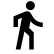
\includegraphics[scale=0.5]{capitulo-6/graphics/ic_activity_walk} & \emph{WALKING} & Caminar\tabularnewline
\hline 
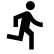
\includegraphics[scale=0.5]{capitulo-6/graphics/ic_activity_run} & \emph{RUNNING} & Trotar\tabularnewline
\hline 
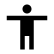
\includegraphics[scale=0.5]{capitulo-6/graphics/ic_activity_still} & \emph{STILL} & Estar quieto\tabularnewline
\hline 
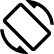
\includegraphics[scale=0.5]{capitulo-6/graphics/ic_activity_tilt} & \emph{TILTING} & Estar inquieto\tabularnewline
\hline 
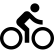
\includegraphics[scale=0.5]{capitulo-6/graphics/ic_activity_bike} & \emph{ON BICYCLE}  & Andar en bicicleta\tabularnewline
\hline 
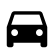
\includegraphics[scale=0.5]{capitulo-6/graphics/ic_activity_car} & \emph{IN VEHICLE}  & \multirow{1}{*}{Andar en automóvil}\tabularnewline
\hline 
\end{tabular}
\par\end{centering}
\caption{\label{tab6:etiquetas}Actividades humanas etiquetadas}
\end{table}

El resultado del experimento se resume en la \tabref{tab6:sesiones},
aquí se incluyen las sesiones hechas por los voluntarios y el tiempo
en minutos acumulado que fue invertido en cada actividad. 

\begin{table}[h]
\begin{centering}
\begin{tabular}{|c|c|c|c|c|c|c|}
\hline 
\multirow{2}{*}{Individuo} & \multicolumn{6}{c|}{Actividades}\tabularnewline
\cline{2-7} 
 & \emph{\footnotesize{}WALKING} & \emph{\footnotesize{}RUNNING} & \emph{\footnotesize{}STILL} & \emph{\footnotesize{}TILTING} & \emph{\footnotesize{}ON BICYLE} & \emph{\footnotesize{}IN VEHICLE}\tabularnewline
\hline 
\hline 
AG & 80 & 33 & 12 & 10 & 17 & 7\tabularnewline
\hline 
SG & 15 & 15 & - & - & - & -\tabularnewline
\hline 
SF & 43 & 25 & - & - & 13 & -\tabularnewline
\hline 
GA & 30 & 2 & - & - & - & -\tabularnewline
\hline 
BV & - & 17 & - & - & - & -\tabularnewline
\hline 
PV & 17 & 19 & 12 & - & - & 7\tabularnewline
\hline 
SY & 37 & 13 &  & 10 & 26 & 11\tabularnewline
\hline 
MD & 29 & 4 & - & - & - & -\tabularnewline
\hline 
\end{tabular}
\par\end{centering}
\caption{\label{tab6:sesiones}Resumen de sesiones de entrenamiento}
\end{table}


\subsection{Captura de Datos}

El experimento requiere de una cantidad de datos recolectados de los
voluntarios mientras realizan las actividades humanas dictadas durante
el entrenamiento. \emph{SensorLog} \cite{Alan2014s} es una aplicación
\abbr{Android} que se utilizó para la captura y persistencia de las
señales del sensor de aceleración como se ve en la \figref{fig4:sensor-log}.
La aplicación permite exportar las señales de sensores almacenadas
en forma agrupada por sesiones y subirlas a la nube. En la \tabref{tab6:captura}
se resumen las cantidades de medidas de señales capturadas.

\begin{table}[h]
\begin{centering}
\begin{tabular}{|c|c|c|c|c|c|}
\hline 
\multicolumn{6}{|c|}{Actividades}\tabularnewline
\hline 
\emph{\footnotesize{}WALKING} & \emph{\footnotesize{}RUNNING} & \emph{\footnotesize{}STILL} & \emph{\footnotesize{}TILTING} & \emph{\footnotesize{}ON BICYLE} & \emph{\footnotesize{}IN VEHICLE}\tabularnewline
\hline 
\hline 
3.591.788 & 1.604.270 & 387.735 & 134.566 & 819.992 & 365.814\tabularnewline
\hline 
\end{tabular}
\par\end{centering}
\caption{\label{tab6:captura}Unidades de datos capturados}
\end{table}


\subsection{Conjunto de Entrenamiento }

En la \tabref{tab6:muestras} se resumen las cantidades de las muestras
calculadas de acuerdo lo descrito en el proceso de la \secref{ssec44:extraction}.

\begin{table}[h]
\begin{centering}
\begin{tabular}{|c|c|c|c|c|c|}
\hline 
\multicolumn{6}{|c|}{Actividades}\tabularnewline
\hline 
\emph{\footnotesize{}WALKING} & \emph{\footnotesize{}RUNNING} & \emph{\footnotesize{}STILL} & \emph{\footnotesize{}TILTING} & \emph{\footnotesize{}ON BICYLE} & \emph{\footnotesize{}IN VEHICLE}\tabularnewline
\hline 
\hline 
5.915 & 3.019 & 645 & 485 & 1.338 & 610\tabularnewline
\hline 
\end{tabular}
\par\end{centering}
\caption{\label{tab6:muestras}Unidades de muestras procesadas}
\end{table}

El proceso de generación del clasificador está automatizado por medio
del flujo mostrado en la \figref{fig6:proceso-clasi}.

\begin{figure}[th]
\begin{centering}
\includegraphics[width=0.8\textwidth]{\string"capitulo-6/graphics/Proceso de Clasificacion\string".png}
\par\end{centering}
\caption{\label{fig6:proceso-clasi}Flujo de generación del clasificador C4.5}
\end{figure}


\section{Clasificador de Actividades Humanas}

\label{sec6:clasificacion}Un clasificador de actividades humanas
es un clasificador de clases discretas que utiliza un algoritmo de
aprendizaje automático supervisado basado en árboles de decisión.
Este clasificador evalúa como entrada una instancia sin etiquetar
obtenida a partir de datos observados y produce como salida una predicción
de la etiqueta más probable asociada en base a observaciones previas.

En esta sección se describe el procedimiento de generación de un clasificador
\abbr{HAR} utilizando un conjunto de entrenamiento inicial. Luego
se evalúa el mismo por medio de pruebas y verificación para garantizar
su efectividad. Este procedimiento se realiza utilizando la herramienta
de aprendizaje automático denominado \emph{Waikato Environment Knowledge
Analysis} \texttt{(\abbr{WEKA})} \cite{Frank2016}. 

\subsection{Métricas de predicción numérica}

De manera a evaluar el rendimiento de los clasificadores de aprendizaje
automático supervisado se describen las siguientes medidas y métricas
de predicción numéricas que dan una noción de cuánto se acercan las
predicciones a los datos observados \cite{Witten2017}.

Utilizando la siguiente nomenclatura de la definición \ref{def3:clasificacion}
de la \secref{sec3:aprendizaje} en que $\hat{f}(x_{i})$ corresponde
a los valores de la predicción de una instancia de evaluación $x_{i}$
e $y_{i}$ corresponde al valor actual de la \emph{$i$-ésima} instancia,
se define cuanto sigue:
\begin{itemize}
\item \emph{Número de instancias}: es el tamaño de la población de entrada
$N$.
\item \emph{Instancias correctamente clasificadas}: es una proporción del
tamaño de la población de entrada $C$.
\item \emph{Instancias incorrectamente clasificadas}: es un proporción del
tamaño de la población de entrada $I$.
\item \emph{Estadísticas Kappa}: es el coeficiente \emph{kappa} de \emph{Cohen}
que establece el valor de coeficiente de concordancia para confiabilidad
de los datos. 
\[
\kappa\text{=}\frac{p_{o}-p_{e}}{1-p_{e}}
\]
, donde $p_{o}$ es el acuerdo observado relativo y $p_{e}$ es la
probabilidad hipotética de acuerdo. Los valores se dividen en los
siguientes rangos.\\
\\
\begin{tabular}{|c|c|c|}
\hline 
Valor & Nivel de acuerdo & \% de datos confiables\tabularnewline
\hline 
\hline 
0 - 0.20 & No & 0 - 4\%\tabularnewline
\hline 
0.21 - 0.39 & Mínimo & 4 - 15\%\tabularnewline
\hline 
0.40 - 0.59 & Débil & 15 - 35\%\tabularnewline
\hline 
0.60 - 0.79 & Moderado & 35 - 63\%\tabularnewline
\hline 
0.80 - 0.90 & Fuerte & 64 - 81\%\tabularnewline
\hline 
>0.90 & Casi perfecto & 82 - 100\%\tabularnewline
\hline 
\end{tabular}
\item \emph{Error medio absoluto}: es el promedio de la magnitud de los
errores absolutos individuales.
\[
\frac{1}{n}\sum_{i\text{=1}}^{n}\bigl|y_{i}-\hat{f}(x_{i})\bigr|
\]
\item \emph{Raíz de Error cuadrático medio}: es la raíz del promedio de
la magnitud de los errores individuales elevados al cuadrado.
\[
\sqrt{\frac{1}{n}\sum_{i\text{=1}}^{n}\left(y_{i}-\hat{f}(x_{i})\right)^{2}}
\]
\item \emph{Error absoluto relativo}: es la razón de la suma de los errores
absolutos y la suma de las diferencia absoluta de los valores exactos
con la media. 
\[
\sum_{i\text{=1}}^{n}\frac{\bigl|y_{i}-\hat{f}(x_{i})\bigr|}{\bigl|y_{i}-\bar{y}\bigr|}\,\textrm{, donde\,}\bar{y}=\frac{1}{n}\sum_{i=1}^{n}y_{i}
\]
\item \emph{Raíz de Error cuadrático relativo}: es la raíz de la razón de
la suma de los errores individuales elevados al cuadrado y la suma
de las diferencia de los valores exactos con la media elevados al
cuadrado. 
\[
\sqrt{\sum_{i\text{=1}}^{n}\frac{\left(y-\hat{f}(x_{i})\right)^{2}}{\left(y_{i}-\bar{y_{i}}\right)^{2}}}
\]
\end{itemize}

\subsection{Evaluación del clasificador}

El clasificador generado en este trabajo es un árbol de decisión obtenido
por medio del algoritmo C4.5 (\algref{algoC45}) y la implementación
en \emph{Java} J48 \cite{Frank2016b}. El tamaño del árbol generado
es de $677$ nodos, de los cuales $339$ corresponden a hojas.

A continuación se presentan las métricas numéricas de predicción del
clasificador generado con las muestras de entrenamiento recolectadas
y descritas anteriormente: 
\begin{itemize}
\item Número de instancias: $12.012$ 
\item Instancias correctamente clasificadas: $10.942$ (en porcentaje $91,0922$
\%)
\item Instancias incorrectamente clasificadas: $1.070$ (en porcentaje $8,9078$
\%)
\item Estadísticas Kappa: $0,8678$ 
\item Error medio absoluto: $0,0341$
\item Raíz de Error cuadrático medio: $0,164$ 
\item Error absoluto relativo: $15,1717$ \% 
\item Raíz de Error cuadrático relativo: $48,9126$ \% 
\end{itemize}
En general, se puede apreciar que la taza de errorres es baja, la
cantidad de instancias correctas alta y el coeficiente de confianza
es fuerte. Adicionalmente, en la \tabref{tab6:matriz-confusion} se
muestra la matriz de confusión obtenida así como se detalla en la
\secref{sec3:metricas}. 

\begin{table}[h]
\begin{centering}
\begin{tabular}{|l|c|c|c|c|c|c|}
\cline{2-7} 
\multicolumn{1}{l|}{} & \multicolumn{6}{c|}{Matriz de Confusión}\tabularnewline
\hline 
Actividad & \emph{\footnotesize{}WALKING} & \emph{\footnotesize{}RUNNING} & \emph{\footnotesize{}STILL} & \emph{\footnotesize{}TILTING} & \emph{\footnotesize{}ON BICYLE} & \emph{\footnotesize{}ON VEHICLE}\tabularnewline
\hline 
\hline 
\emph{\footnotesize{}WALKING} & 5.643 & 63 & 21 & 28 & 156 & 4\tabularnewline
\hline 
\emph{\footnotesize{}RUNNING} & 122 & 2.852 & 3 & 6 & 36 & 0\tabularnewline
\hline 
\emph{\footnotesize{}STILL} & 19 & 14 & 555 & 23 & 15 & 19\tabularnewline
\hline 
\emph{\footnotesize{}TILTING} & 26 & 3 & 21 & 304 & 46 & 85\tabularnewline
\hline 
\emph{\footnotesize{}ON BICYLE} & 157 & 28 & 7 & 47 & 1.089 & 10\tabularnewline
\hline 
\emph{\footnotesize{}ON VEHICLE} & 2 & 2 & 14 & 86 & 7 & 499\tabularnewline
\hline 
\end{tabular}
\par\end{centering}
\caption{\label{tab6:matriz-confusion}Matriz de confusión del clasificador
resultante}
\end{table}

A partir de esta matriz se obtuvieron los siguientes calculos de métricas
de evaluación para clasificadores expuesto también en la \secref{sec3:metricas}:
\begin{itemize}
\item Precisión: $0,9174$
\item Exhaustividad: $0,9109$
\item Exactitud: $0,9714$
\item \emph{Valor-F}: $0,9142$
\end{itemize}
Finalmente, se puede apreciar que los valores demuestran una buena
efectividad del clasificador generado debido a que las métricas están
por encima de 90\%.

\section{Resultados Experimentales}

\label{sec6:resultados}Describir resultados de experimento con HARDroid.
